\documentclass[tikz]{standalone}
\standaloneconfig{border=1cm} 
\usepackage[utf8]{inputenc}

\usetikzlibrary{positioning}
\usetikzlibrary{shapes}
\usetikzlibrary{matrix}
\usetikzlibrary{backgrounds}
\usetikzlibrary{calc}

\title{Autoencoder}
\author{James Allingham}
\date{August 2019}

\begin{document}
	
\tikzset{arrow/.style={-stealth, thick, draw=gray!80!black}}

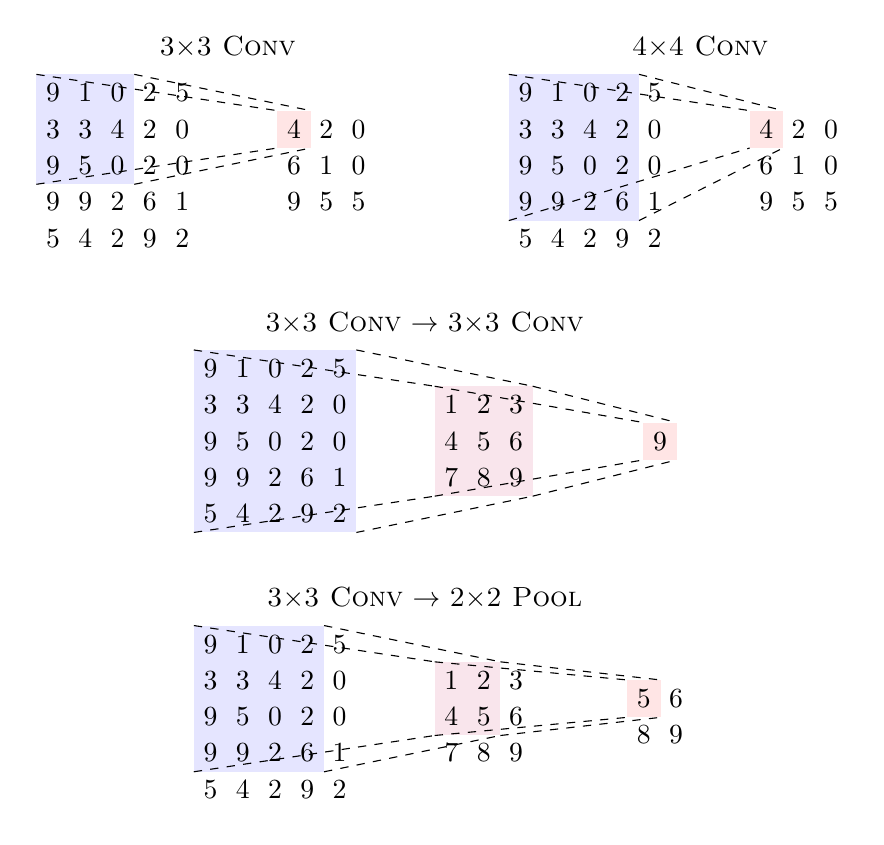
\begin{tikzpicture}[ampersand replacement=\&]
%     \draw[help lines](0,-5) grid (10,5);  
     
    %%%% 3x3 Conv %%%%
	
	\matrix (A1) [matrix of math nodes, yslant=-50, xslant=-50] at (-2,0)
	{
		9 \& 1 \& 0 \& 2 \& 5 \\
		3 \& 3 \& 4 \& 2 \& 0 \\
		9 \& 5 \& 0 \& 2 \& 0 \\
		9 \& 9 \& 2 \& 6 \& 1 \\
		5 \& 4 \& 2 \& 9 \& 2 \\
	};
	
	\begin{scope}[on background layer]
	\fill[blue!10] (A1-1-1.west|-A1-1-1.north) rectangle (A1-3-3.south-|A1-3-3.east); 
	\end{scope}
	
	\node[] at ($(A1.east)+(0.25,1.5)$) {\textsc{3$\times$3 Conv}};
	
	\matrix (B1) [matrix of math nodes, yslant=-50, xslant=-50] at ($(A1.east)+(1.5,0)$)
	{
		4 \& 2 \& 0 \\
		6 \& 1 \& 0 \\
		9 \& 5 \& 5 \\
	};
	\begin{scope}[on background layer]
	\fill[red!10] (B1-1-1.west|-B1-1-1.north) rectangle (B1-1-1.south-|B1-1-1.east); 
	\end{scope}
	
	\path[-,dashed] (A1-1-1.west|-A1-1-1.north) edge (B1-1-1.west|-B1-1-1.north);
	\path[-,dashed] (A1-1-3.east|-A1-1-3.north) edge (B1-1-1.east|-B1-1-1.north);
	\path[-,dashed] (A1-3-1.west|-A1-3-1.south) edge (B1-1-1.west|-B1-1-1.south);
	\path[-,dashed] (A1-3-3.east|-A1-3-3.south) edge (B1-1-1.east|-B1-1-1.south);
	
	%%% 4x4 Conv %%%
	
	\matrix (A2) [matrix of math nodes, yslant=-50, xslant=-50] at (4,0)
	{
		9 \& 1 \& 0 \& 2 \& 5 \\
		3 \& 3 \& 4 \& 2 \& 0 \\
		9 \& 5 \& 0 \& 2 \& 0 \\
		9 \& 9 \& 2 \& 6 \& 1 \\
		5 \& 4 \& 2 \& 9 \& 2 \\
	};
	
	\begin{scope}[on background layer]
	\fill[blue!10] (A2-1-1.west|-A2-1-1.north) rectangle (A2-4-4.south-|A2-4-4.east); 
	\end{scope}
	
	\node[] at ($(A2.east)+(0.25,1.5)$) {\textsc{4$\times$4 Conv}};
	
	\matrix (B2) [matrix of math nodes, yslant=-50, xslant=-50] at ($(A2.east)+(1.5,0)$)
	{
		4 \& 2 \& 0 \\
		6 \& 1 \& 0 \\
		9 \& 5 \& 5 \\
	};
	\begin{scope}[on background layer]
	\fill[red!10] (B2-1-1.west|-B2-1-1.north) rectangle (B2-1-1.south-|B2-1-1.east); 
	\end{scope}
	
	\path[-,dashed] (A2-1-1.west|-A2-1-1.north) edge (B2-1-1.west|-B2-1-1.north);
	\path[-,dashed] (A2-1-4.east|-A2-1-4.north) edge (B2-1-1.east|-B2-1-1.north);
	\path[-,dashed] (A2-4-1.west|-A2-4-1.south) edge (B2-1-1.west|-B2-1-1.south);
	\path[-,dashed] (A2-4-4.east|-A2-4-4.south) edge (B2-1-1.east|-B2-1-1.south);
	
	%%% 3x3 -> 3x3 %%%
	
	\matrix (A3) [matrix of math nodes, yslant=-50, xslant=-50] at (0,-3.5)
	{
		9 \& 1 \& 0 \& 2 \& 5 \\
		3 \& 3 \& 4 \& 2 \& 0 \\
		9 \& 5 \& 0 \& 2 \& 0 \\
		9 \& 9 \& 2 \& 6 \& 1 \\
		5 \& 4 \& 2 \& 9 \& 2 \\
	};
	
	\begin{scope}[on background layer]
	\fill[blue!10] (A3-1-1.west|-A3-1-1.north) rectangle (A3-5-5.south-|A3-5-5.east); 
	\end{scope}
	
	\node[] at ($(A3.east)+(0.75,1.5)$) {\textsc{3$\times$3 Conv} $\rightarrow$ \textsc{3$\times$3 Conv}};
	
	\matrix (B3) [matrix of math nodes, yslant=-50, xslant=-50] at ($(A3.east)+(1.5,0)$)
	{
		1 \& 2 \& 3 \\
		4 \& 5 \& 6 \\
		7 \& 8 \& 9 \\
	};
	
	\begin{scope}[on background layer]
	\fill[purple!10] (B3-1-1.west|-B3-1-1.north) rectangle (B3-3-3.south-|B3-3-3.east); 
	\end{scope}
	
	\path[-,dashed] (A3-1-1.west|-A3-1-1.north) edge (B3-1-1.west|-B3-1-1.north);
	\path[-,dashed] (A3-1-5.east|-A3-1-5.north) edge (B3-1-3.east|-B3-1-3.north);
	\path[-,dashed] (A3-5-1.west|-A3-5-1.south) edge (B3-3-1.west|-B3-3-1.south);
	\path[-,dashed] (A3-5-5.east|-A3-5-5.south) edge (B3-3-3.east|-B3-3-3.south);
	
	\matrix (C3) [matrix of math nodes, yslant=-50, xslant=-50] at ($(B3.east)+(1.5,0)$)
	{
		9 \\
	};
	\begin{scope}[on background layer]
	\fill[red!10] (C3-1-1.west|-C3-1-1.north) rectangle (C3-1-1.south-|C3-1-1.east); 
	\end{scope}
	
	\path[-,dashed] (B3-1-1.west|-B3-1-1.north) edge (C3-1-1.west|-C3-1-1.north);
	\path[-,dashed] (B3-1-3.east|-B3-1-3.north) edge (C3-1-1.east|-C3-1-1.north);
	\path[-,dashed] (B3-3-1.west|-B3-3-1.south) edge (C3-1-1.west|-C3-1-1.south);
	\path[-,dashed] (B3-3-3.east|-B3-3-3.south) edge (C3-1-1.east|-C3-1-1.south);
	
	%%% 3x3 -> 2x2
	
	\matrix (A4) [matrix of math nodes, yslant=-50, xslant=-50] at (0,-7)
	{
		9 \& 1 \& 0 \& 2 \& 5 \\
		3 \& 3 \& 4 \& 2 \& 0 \\
		9 \& 5 \& 0 \& 2 \& 0 \\
		9 \& 9 \& 2 \& 6 \& 1 \\
		5 \& 4 \& 2 \& 9 \& 2 \\
	};
	
	\begin{scope}[on background layer]
	\fill[blue!10] (A4-1-1.west|-A4-1-1.north) rectangle (A4-4-4.south-|A4-4-4.east); 
	\end{scope}
	
	\node[] at ($(A4.east)+(0.75,1.5)$) {\textsc{3$\times$3 Conv} $\rightarrow$ \textsc{2$\times$2 Pool}};
	
	\matrix (B4) [matrix of math nodes, yslant=-50, xslant=-50] at ($(A4.east)+(1.5,0)$)
	{
		1 \& 2 \& 3 \\
		4 \& 5 \& 6 \\
		7 \& 8 \& 9 \\
	};
	
	\begin{scope}[on background layer]
	\fill[purple!10] (B4-1-1.west|-B4-1-1.north) rectangle (B4-2-2.south-|B4-2-2.east); 
	\end{scope}
	
	\path[-,dashed] (A4-1-1.west|-A4-1-1.north) edge (B4-1-1.west|-B4-1-1.north);
	\path[-,dashed] (A4-1-4.east|-A4-1-4.north) edge (B4-1-2.east|-B4-1-2.north);
	\path[-,dashed] (A4-4-1.west|-A4-4-1.south) edge (B4-2-1.west|-B4-2-1.south);
	\path[-,dashed] (A4-4-4.east|-A4-4-4.south) edge (B4-2-2.east|-B4-2-2.south);
	
	\matrix (C4) [matrix of math nodes, yslant=-50, xslant=-50] at ($(B4.east)+(1.5,0)$)
	{
		5 \& 6\\
		8 \& 9\\
	};
	\begin{scope}[on background layer]
	\fill[red!10] (C4-1-1.west|-C4-1-1.north) rectangle (C4-1-1.south-|C4-1-1.east); 
	\end{scope}
	
	\path[-,dashed] (B4-1-1.west|-B4-1-1.north) edge (C4-1-1.west|-C4-1-1.north);
	\path[-,dashed] (B4-1-2.east|-B4-1-2.north) edge (C4-1-1.east|-C4-1-1.north);
	\path[-,dashed] (B4-2-1.west|-B4-2-1.south) edge (C4-1-1.west|-C4-1-1.south);
	\path[-,dashed] (B4-2-2.east|-B4-2-2.south) edge (C4-1-1.east|-C4-1-1.south);	
     
\end{tikzpicture}

\end{document}